% Created by tikzDevice version 0.7.0 on 2014-07-26 02:55:52
% !TEX encoding = UTF-8 Unicode
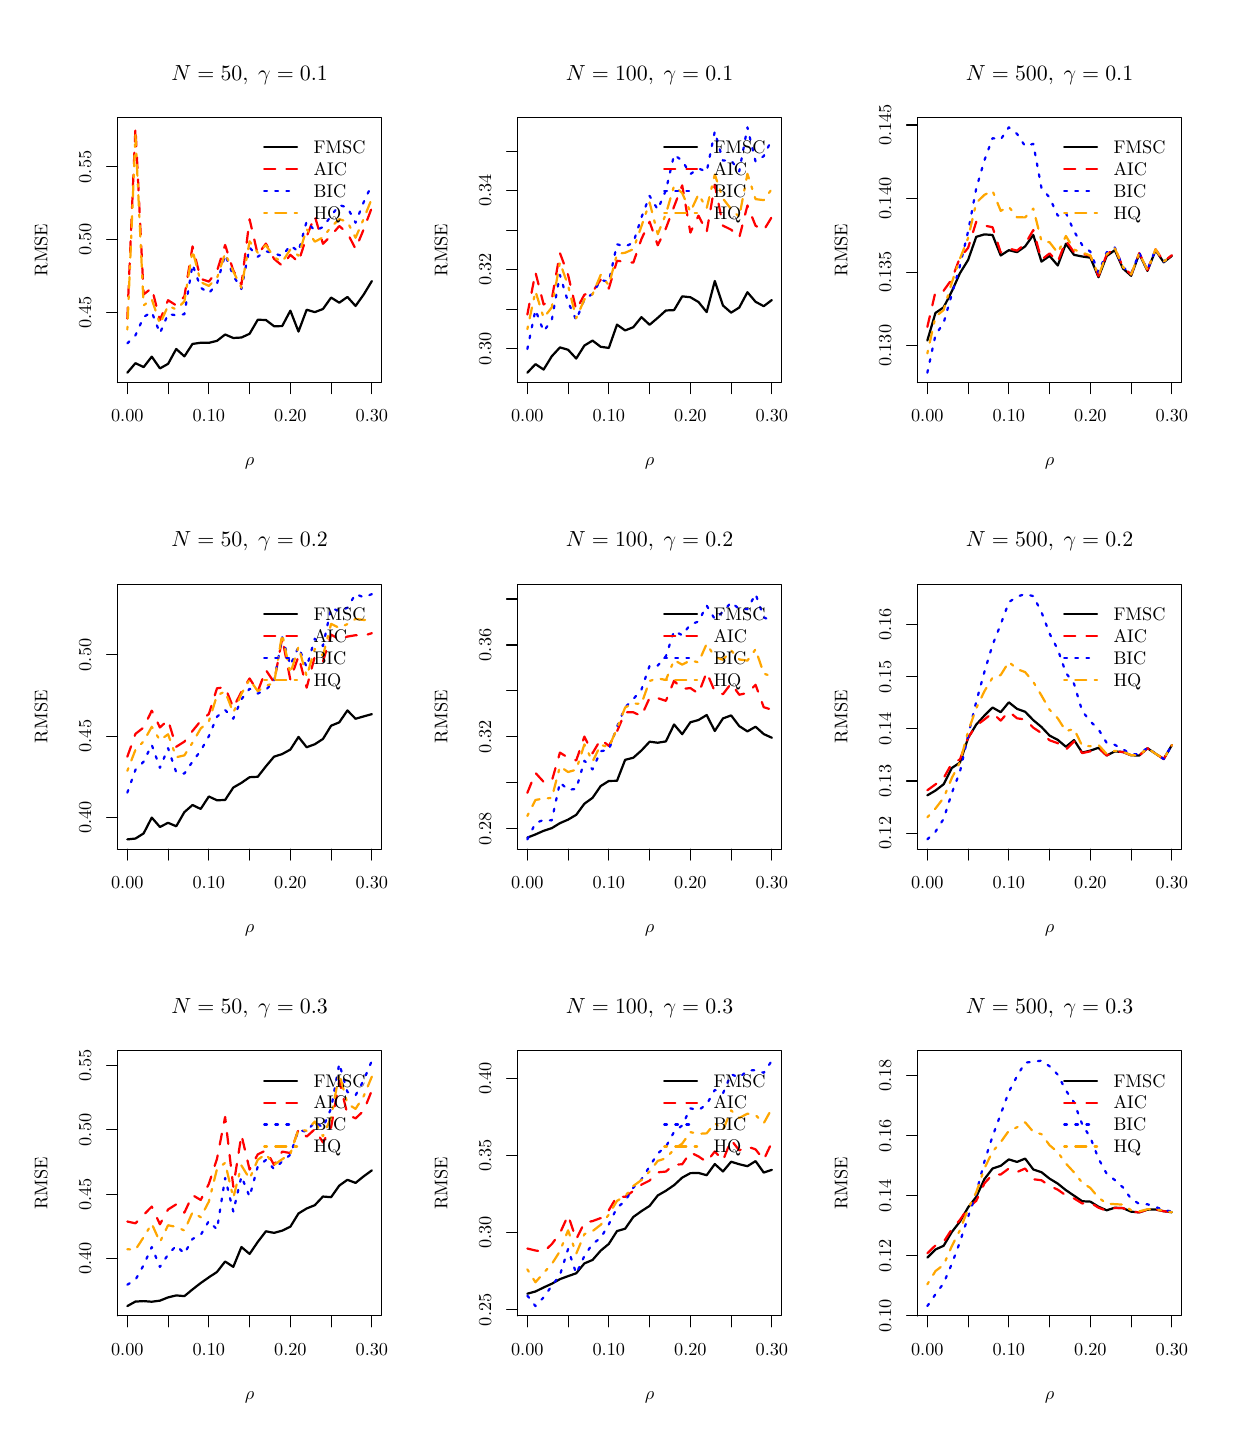
\begin{tikzpicture}[x=1pt,y=1pt]
\definecolor[named]{fillColor}{rgb}{1.00,1.00,1.00}
\path[use as bounding box,fill=fillColor,fill opacity=0.00] (0,0) rectangle (433.62,505.89);
\begin{scope}
\path[clip] ( 32.47,377.65) rectangle (127.91,473.42);
\definecolor[named]{drawColor}{rgb}{0.00,0.00,0.00}

\path[draw=drawColor,line width= 0.8pt,line join=round,line cap=round] ( 36.01,381.20) --
	( 38.95,384.66) --
	( 41.90,383.22) --
	( 44.84,387.01) --
	( 47.79,382.77) --
	( 50.73,384.39) --
	( 53.68,389.78) --
	( 56.63,387.12) --
	( 59.57,391.61) --
	( 62.52,392.03) --
	( 65.46,392.00) --
	( 68.41,392.72) --
	( 71.35,395.02) --
	( 74.30,393.75) --
	( 77.24,393.92) --
	( 80.19,395.28) --
	( 83.14,400.34) --
	( 86.08,400.26) --
	( 89.03,398.00) --
	( 91.97,398.05) --
	( 94.92,403.64) --
	( 97.86,396.07) --
	(100.81,403.97) --
	(103.75,403.10) --
	(106.70,404.22) --
	(109.65,408.36) --
	(112.59,406.50) --
	(115.54,408.58) --
	(118.48,405.32) --
	(121.43,409.47) --
	(124.37,414.32);
\end{scope}
\begin{scope}
\path[clip] (  0.00,  0.00) rectangle (433.62,505.89);
\definecolor[named]{drawColor}{rgb}{0.00,0.00,0.00}

\path[draw=drawColor,line width= 0.4pt,line join=round,line cap=round] ( 36.01,377.65) -- (124.37,377.65);

\path[draw=drawColor,line width= 0.4pt,line join=round,line cap=round] ( 36.01,377.65) -- ( 36.01,373.69);

\path[draw=drawColor,line width= 0.4pt,line join=round,line cap=round] ( 50.73,377.65) -- ( 50.73,373.69);

\path[draw=drawColor,line width= 0.4pt,line join=round,line cap=round] ( 65.46,377.65) -- ( 65.46,373.69);

\path[draw=drawColor,line width= 0.4pt,line join=round,line cap=round] ( 80.19,377.65) -- ( 80.19,373.69);

\path[draw=drawColor,line width= 0.4pt,line join=round,line cap=round] ( 94.92,377.65) -- ( 94.92,373.69);

\path[draw=drawColor,line width= 0.4pt,line join=round,line cap=round] (109.65,377.65) -- (109.65,373.69);

\path[draw=drawColor,line width= 0.4pt,line join=round,line cap=round] (124.37,377.65) -- (124.37,373.69);

\node[text=drawColor,anchor=base,inner sep=0pt, outer sep=0pt, scale=  0.66] at ( 36.01,363.40) {0.00};

\node[text=drawColor,anchor=base,inner sep=0pt, outer sep=0pt, scale=  0.66] at ( 65.46,363.40) {0.10};

\node[text=drawColor,anchor=base,inner sep=0pt, outer sep=0pt, scale=  0.66] at ( 94.92,363.40) {0.20};

\node[text=drawColor,anchor=base,inner sep=0pt, outer sep=0pt, scale=  0.66] at (124.37,363.40) {0.30};

\path[draw=drawColor,line width= 0.4pt,line join=round,line cap=round] ( 32.47,403.08) -- ( 32.47,455.58);

\path[draw=drawColor,line width= 0.4pt,line join=round,line cap=round] ( 32.47,403.08) -- ( 28.51,403.08);

\path[draw=drawColor,line width= 0.4pt,line join=round,line cap=round] ( 32.47,429.33) -- ( 28.51,429.33);

\path[draw=drawColor,line width= 0.4pt,line join=round,line cap=round] ( 32.47,455.58) -- ( 28.51,455.58);

\node[text=drawColor,rotate= 90.00,anchor=base,inner sep=0pt, outer sep=0pt, scale=  0.66] at ( 22.97,403.08) {0.45};

\node[text=drawColor,rotate= 90.00,anchor=base,inner sep=0pt, outer sep=0pt, scale=  0.66] at ( 22.97,429.33) {0.50};

\node[text=drawColor,rotate= 90.00,anchor=base,inner sep=0pt, outer sep=0pt, scale=  0.66] at ( 22.97,455.58) {0.55};

\path[draw=drawColor,line width= 0.4pt,line join=round,line cap=round] ( 32.47,377.65) --
	(127.91,377.65) --
	(127.91,473.42) --
	( 32.47,473.42) --
	( 32.47,377.65);
\end{scope}
\begin{scope}
\path[clip] (  0.00,337.26) rectangle (144.54,505.89);
\definecolor[named]{drawColor}{rgb}{0.00,0.00,0.00}

\node[text=drawColor,anchor=base,inner sep=0pt, outer sep=0pt, scale=  0.79] at ( 80.19,486.92) {\bfseries $N=50, \;\gamma=0.1$};

\node[text=drawColor,anchor=base,inner sep=0pt, outer sep=0pt, scale=  0.66] at ( 80.19,347.56) {$\rho$};

\node[text=drawColor,rotate= 90.00,anchor=base,inner sep=0pt, outer sep=0pt, scale=  0.66] at (  7.13,425.53) {RMSE};
\end{scope}
\begin{scope}
\path[clip] ( 32.47,377.65) rectangle (127.91,473.42);
\definecolor[named]{drawColor}{rgb}{1.00,0.00,0.00}

\path[draw=drawColor,line width= 0.8pt,dash pattern=on 4pt off 4pt ,line join=round,line cap=round] ( 36.01,400.76) --
	( 38.95,469.87) --
	( 41.90,409.50) --
	( 44.84,411.80) --
	( 47.79,400.24) --
	( 50.73,407.40) --
	( 53.68,405.53) --
	( 56.63,408.76) --
	( 59.57,426.85) --
	( 62.52,415.14) --
	( 65.46,414.12) --
	( 68.41,417.94) --
	( 71.35,427.37) --
	( 74.30,418.11) --
	( 77.24,413.01) --
	( 80.19,436.64) --
	( 83.14,423.90) --
	( 86.08,427.86) --
	( 89.03,422.35) --
	( 91.97,419.86) --
	( 94.92,423.81) --
	( 97.86,421.18) --
	(100.81,430.42) --
	(103.75,437.82) --
	(106.70,427.78) --
	(109.65,430.77) --
	(112.59,434.21) --
	(115.54,431.69) --
	(118.48,425.92) --
	(121.43,433.04) --
	(124.37,440.90);
\definecolor[named]{drawColor}{rgb}{0.00,0.00,1.00}

\path[draw=drawColor,line width= 0.8pt,dash pattern=on 1pt off 3pt ,line join=round,line cap=round] ( 36.01,391.81) --
	( 38.95,394.71) --
	( 41.90,401.34) --
	( 44.84,403.14) --
	( 47.79,395.45) --
	( 50.73,402.42) --
	( 53.68,401.95) --
	( 56.63,402.35) --
	( 59.57,420.30) --
	( 62.52,411.96) --
	( 65.46,409.92) --
	( 68.41,413.35) --
	( 71.35,423.82) --
	( 74.30,416.24) --
	( 77.24,411.46) --
	( 80.19,426.45) --
	( 83.14,423.10) --
	( 86.08,425.12) --
	( 89.03,424.29) --
	( 91.97,423.40) --
	( 94.92,427.19) --
	( 97.86,424.99) --
	(100.81,435.93) --
	(103.75,432.50) --
	(106.70,433.83) --
	(109.65,437.87) --
	(112.59,441.78) --
	(115.54,440.91) --
	(118.48,435.40) --
	(121.43,442.88) --
	(124.37,449.14);
\definecolor[named]{drawColor}{rgb}{1.00,0.65,0.00}

\path[draw=drawColor,line width= 0.8pt,dash pattern=on 1pt off 3pt on 4pt off 3pt ,line join=round,line cap=round] ( 36.01,396.83) --
	( 38.95,467.06) --
	( 41.90,405.53) --
	( 44.84,407.83) --
	( 47.79,398.79) --
	( 50.73,405.42) --
	( 53.68,404.06) --
	( 56.63,406.97) --
	( 59.57,425.43) --
	( 62.52,413.94) --
	( 65.46,412.57) --
	( 68.41,415.39) --
	( 71.35,424.38) --
	( 74.30,417.75) --
	( 77.24,411.91) --
	( 80.19,428.69) --
	( 83.14,424.60) --
	( 86.08,427.31) --
	( 89.03,422.91) --
	( 91.97,421.25) --
	( 94.92,425.72) --
	( 97.86,423.51) --
	(100.81,433.14) --
	(103.75,428.54) --
	(106.70,430.10) --
	(109.65,433.88) --
	(112.59,436.69) --
	(115.54,435.76) --
	(118.48,429.97) --
	(121.43,436.82) --
	(124.37,444.20);
\definecolor[named]{drawColor}{rgb}{0.00,0.00,0.00}

\path[draw=drawColor,line width= 0.8pt,line join=round,line cap=round] ( 85.47,462.63) -- ( 97.35,462.63);
\definecolor[named]{drawColor}{rgb}{1.00,0.00,0.00}

\path[draw=drawColor,line width= 0.8pt,dash pattern=on 4pt off 4pt ,line join=round,line cap=round] ( 85.47,454.71) -- ( 97.35,454.71);
\definecolor[named]{drawColor}{rgb}{0.00,0.00,1.00}

\path[draw=drawColor,line width= 0.8pt,dash pattern=on 1pt off 3pt ,line join=round,line cap=round] ( 85.47,446.79) -- ( 97.35,446.79);
\definecolor[named]{drawColor}{rgb}{1.00,0.65,0.00}

\path[draw=drawColor,line width= 0.8pt,dash pattern=on 1pt off 3pt on 4pt off 3pt ,line join=round,line cap=round] ( 85.47,438.87) -- ( 97.35,438.87);
\definecolor[named]{drawColor}{rgb}{0.00,0.00,0.00}

\node[text=drawColor,anchor=base west,inner sep=0pt, outer sep=0pt, scale=  0.66] at (103.29,460.35) {FMSC};

\node[text=drawColor,anchor=base west,inner sep=0pt, outer sep=0pt, scale=  0.66] at (103.29,452.43) {AIC};

\node[text=drawColor,anchor=base west,inner sep=0pt, outer sep=0pt, scale=  0.66] at (103.29,444.51) {BIC};

\node[text=drawColor,anchor=base west,inner sep=0pt, outer sep=0pt, scale=  0.66] at (103.29,436.59) {HQ};
\end{scope}
\begin{scope}
\path[clip] (177.01,377.65) rectangle (272.45,473.42);
\definecolor[named]{drawColor}{rgb}{0.00,0.00,0.00}

\path[draw=drawColor,line width= 0.8pt,line join=round,line cap=round] (180.55,381.20) --
	(183.49,384.30) --
	(186.44,382.35) --
	(189.38,387.14) --
	(192.33,390.35) --
	(195.27,389.50) --
	(198.22,386.33) --
	(201.17,391.02) --
	(204.11,392.81) --
	(207.06,390.57) --
	(210.00,390.16) --
	(212.95,398.58) --
	(215.89,396.48) --
	(218.84,397.65) --
	(221.78,401.28) --
	(224.73,398.53) --
	(227.68,401.04) --
	(230.62,403.70) --
	(233.57,403.82) --
	(236.51,408.80) --
	(239.46,408.48) --
	(242.40,406.75) --
	(245.35,403.11) --
	(248.29,414.34) --
	(251.24,405.49) --
	(254.19,402.91) --
	(257.13,404.76) --
	(260.08,410.29) --
	(263.02,406.83) --
	(265.97,405.25) --
	(268.91,407.47);
\end{scope}
\begin{scope}
\path[clip] (  0.00,  0.00) rectangle (433.62,505.89);
\definecolor[named]{drawColor}{rgb}{0.00,0.00,0.00}

\path[draw=drawColor,line width= 0.4pt,line join=round,line cap=round] (180.55,377.65) -- (268.91,377.65);

\path[draw=drawColor,line width= 0.4pt,line join=round,line cap=round] (180.55,377.65) -- (180.55,373.69);

\path[draw=drawColor,line width= 0.4pt,line join=round,line cap=round] (195.27,377.65) -- (195.27,373.69);

\path[draw=drawColor,line width= 0.4pt,line join=round,line cap=round] (210.00,377.65) -- (210.00,373.69);

\path[draw=drawColor,line width= 0.4pt,line join=round,line cap=round] (224.73,377.65) -- (224.73,373.69);

\path[draw=drawColor,line width= 0.4pt,line join=round,line cap=round] (239.46,377.65) -- (239.46,373.69);

\path[draw=drawColor,line width= 0.4pt,line join=round,line cap=round] (254.19,377.65) -- (254.19,373.69);

\path[draw=drawColor,line width= 0.4pt,line join=round,line cap=round] (268.91,377.65) -- (268.91,373.69);

\node[text=drawColor,anchor=base,inner sep=0pt, outer sep=0pt, scale=  0.66] at (180.55,363.40) {0.00};

\node[text=drawColor,anchor=base,inner sep=0pt, outer sep=0pt, scale=  0.66] at (210.00,363.40) {0.10};

\node[text=drawColor,anchor=base,inner sep=0pt, outer sep=0pt, scale=  0.66] at (239.46,363.40) {0.20};

\node[text=drawColor,anchor=base,inner sep=0pt, outer sep=0pt, scale=  0.66] at (268.91,363.40) {0.30};

\path[draw=drawColor,line width= 0.4pt,line join=round,line cap=round] (177.01,389.84) -- (177.01,461.27);

\path[draw=drawColor,line width= 0.4pt,line join=round,line cap=round] (177.01,389.84) -- (173.05,389.84);

\path[draw=drawColor,line width= 0.4pt,line join=round,line cap=round] (177.01,404.13) -- (173.05,404.13);

\path[draw=drawColor,line width= 0.4pt,line join=round,line cap=round] (177.01,418.41) -- (173.05,418.41);

\path[draw=drawColor,line width= 0.4pt,line join=round,line cap=round] (177.01,432.70) -- (173.05,432.70);

\path[draw=drawColor,line width= 0.4pt,line join=round,line cap=round] (177.01,446.99) -- (173.05,446.99);

\path[draw=drawColor,line width= 0.4pt,line join=round,line cap=round] (177.01,461.27) -- (173.05,461.27);

\node[text=drawColor,rotate= 90.00,anchor=base,inner sep=0pt, outer sep=0pt, scale=  0.66] at (167.51,389.84) {0.30};

\node[text=drawColor,rotate= 90.00,anchor=base,inner sep=0pt, outer sep=0pt, scale=  0.66] at (167.51,418.41) {0.32};

\node[text=drawColor,rotate= 90.00,anchor=base,inner sep=0pt, outer sep=0pt, scale=  0.66] at (167.51,446.99) {0.34};

\path[draw=drawColor,line width= 0.4pt,line join=round,line cap=round] (177.01,377.65) --
	(272.45,377.65) --
	(272.45,473.42) --
	(177.01,473.42) --
	(177.01,377.65);
\end{scope}
\begin{scope}
\path[clip] (144.54,337.26) rectangle (289.08,505.89);
\definecolor[named]{drawColor}{rgb}{0.00,0.00,0.00}

\node[text=drawColor,anchor=base,inner sep=0pt, outer sep=0pt, scale=  0.79] at (224.73,486.92) {\bfseries $N=100, \;\gamma=0.1$};

\node[text=drawColor,anchor=base,inner sep=0pt, outer sep=0pt, scale=  0.66] at (224.73,347.56) {$\rho$};

\node[text=drawColor,rotate= 90.00,anchor=base,inner sep=0pt, outer sep=0pt, scale=  0.66] at (151.67,425.53) {RMSE};
\end{scope}
\begin{scope}
\path[clip] (177.01,377.65) rectangle (272.45,473.42);
\definecolor[named]{drawColor}{rgb}{1.00,0.00,0.00}

\path[draw=drawColor,line width= 0.8pt,dash pattern=on 4pt off 4pt ,line join=round,line cap=round] (180.55,402.21) --
	(183.49,417.45) --
	(186.44,405.86) --
	(189.38,407.78) --
	(192.33,424.44) --
	(195.27,416.57) --
	(198.22,403.93) --
	(201.17,409.42) --
	(204.11,410.40) --
	(207.06,414.81) --
	(210.00,411.61) --
	(212.95,421.65) --
	(215.89,421.33) --
	(218.84,420.98) --
	(221.78,429.51) --
	(224.73,435.75) --
	(227.68,427.25) --
	(230.62,433.38) --
	(233.57,441.25) --
	(236.51,448.89) --
	(239.46,431.84) --
	(242.40,437.95) --
	(245.35,432.04) --
	(248.29,449.15) --
	(251.24,434.35) --
	(254.19,432.89) --
	(257.13,430.06) --
	(260.08,441.65) --
	(263.02,434.32) --
	(265.97,432.66) --
	(268.91,437.52);
\definecolor[named]{drawColor}{rgb}{0.00,0.00,1.00}

\path[draw=drawColor,line width= 0.8pt,dash pattern=on 1pt off 3pt ,line join=round,line cap=round] (180.55,389.75) --
	(183.49,403.90) --
	(186.44,396.18) --
	(189.38,400.21) --
	(192.33,416.54) --
	(195.27,406.72) --
	(198.22,400.24) --
	(201.17,407.69) --
	(204.11,409.71) --
	(207.06,414.70) --
	(210.00,414.07) --
	(212.95,427.62) --
	(215.89,426.82) --
	(218.84,428.16) --
	(221.78,437.31) --
	(224.73,445.09) --
	(227.68,440.17) --
	(230.62,447.13) --
	(233.57,459.92) --
	(236.51,457.85) --
	(239.46,452.97) --
	(242.40,455.00) --
	(245.35,453.88) --
	(248.29,468.35) --
	(251.24,457.85) --
	(254.19,457.96) --
	(257.13,453.96) --
	(260.08,469.87) --
	(263.02,457.50) --
	(265.97,459.47) --
	(268.91,465.54);
\definecolor[named]{drawColor}{rgb}{1.00,0.65,0.00}

\path[draw=drawColor,line width= 0.8pt,dash pattern=on 1pt off 3pt on 4pt off 3pt ,line join=round,line cap=round] (180.55,396.94) --
	(183.49,410.64) --
	(186.44,401.04) --
	(189.38,404.80) --
	(192.33,421.07) --
	(195.27,412.70) --
	(198.22,400.92) --
	(201.17,407.69) --
	(204.11,409.51) --
	(207.06,416.56) --
	(210.00,412.82) --
	(212.95,424.14) --
	(215.89,424.55) --
	(218.84,425.84) --
	(221.78,434.14) --
	(224.73,442.71) --
	(227.68,431.27) --
	(230.62,438.59) --
	(233.57,448.71) --
	(236.51,446.13) --
	(239.46,439.33) --
	(242.40,445.67) --
	(245.35,440.60) --
	(248.29,452.81) --
	(251.24,444.11) --
	(254.19,440.34) --
	(257.13,437.54) --
	(260.08,453.08) --
	(263.02,443.93) --
	(265.97,443.57) --
	(268.91,447.61);
\definecolor[named]{drawColor}{rgb}{0.00,0.00,0.00}

\path[draw=drawColor,line width= 0.8pt,line join=round,line cap=round] (230.01,462.63) -- (241.89,462.63);
\definecolor[named]{drawColor}{rgb}{1.00,0.00,0.00}

\path[draw=drawColor,line width= 0.8pt,dash pattern=on 4pt off 4pt ,line join=round,line cap=round] (230.01,454.71) -- (241.89,454.71);
\definecolor[named]{drawColor}{rgb}{0.00,0.00,1.00}

\path[draw=drawColor,line width= 0.8pt,dash pattern=on 1pt off 3pt ,line join=round,line cap=round] (230.01,446.79) -- (241.89,446.79);
\definecolor[named]{drawColor}{rgb}{1.00,0.65,0.00}

\path[draw=drawColor,line width= 0.8pt,dash pattern=on 1pt off 3pt on 4pt off 3pt ,line join=round,line cap=round] (230.01,438.87) -- (241.89,438.87);
\definecolor[named]{drawColor}{rgb}{0.00,0.00,0.00}

\node[text=drawColor,anchor=base west,inner sep=0pt, outer sep=0pt, scale=  0.66] at (247.83,460.35) {FMSC};

\node[text=drawColor,anchor=base west,inner sep=0pt, outer sep=0pt, scale=  0.66] at (247.83,452.43) {AIC};

\node[text=drawColor,anchor=base west,inner sep=0pt, outer sep=0pt, scale=  0.66] at (247.83,444.51) {BIC};

\node[text=drawColor,anchor=base west,inner sep=0pt, outer sep=0pt, scale=  0.66] at (247.83,436.59) {HQ};
\end{scope}
\begin{scope}
\path[clip] (321.55,377.65) rectangle (416.99,473.42);
\definecolor[named]{drawColor}{rgb}{0.00,0.00,0.00}

\path[draw=drawColor,line width= 0.8pt,line join=round,line cap=round] (325.09,392.84) --
	(328.03,402.83) --
	(330.98,404.81) --
	(333.92,410.59) --
	(336.87,417.17) --
	(339.81,421.93) --
	(342.76,430.31) --
	(345.71,431.19) --
	(348.65,430.97) --
	(351.60,423.57) --
	(354.54,425.47) --
	(357.49,424.77) --
	(360.43,426.85) --
	(363.38,430.99) --
	(366.32,421.35) --
	(369.27,423.41) --
	(372.22,419.95) --
	(375.16,427.81) --
	(378.11,423.78) --
	(381.05,423.20) --
	(384.00,422.78) --
	(386.94,415.71) --
	(389.89,423.35) --
	(392.83,425.49) --
	(395.78,418.86) --
	(398.73,416.23) --
	(401.67,424.15) --
	(404.62,417.99) --
	(407.56,425.46) --
	(410.51,421.10) --
	(413.45,423.42);
\end{scope}
\begin{scope}
\path[clip] (  0.00,  0.00) rectangle (433.62,505.89);
\definecolor[named]{drawColor}{rgb}{0.00,0.00,0.00}

\path[draw=drawColor,line width= 0.4pt,line join=round,line cap=round] (325.09,377.65) -- (413.45,377.65);

\path[draw=drawColor,line width= 0.4pt,line join=round,line cap=round] (325.09,377.65) -- (325.09,373.69);

\path[draw=drawColor,line width= 0.4pt,line join=round,line cap=round] (339.81,377.65) -- (339.81,373.69);

\path[draw=drawColor,line width= 0.4pt,line join=round,line cap=round] (354.54,377.65) -- (354.54,373.69);

\path[draw=drawColor,line width= 0.4pt,line join=round,line cap=round] (369.27,377.65) -- (369.27,373.69);

\path[draw=drawColor,line width= 0.4pt,line join=round,line cap=round] (384.00,377.65) -- (384.00,373.69);

\path[draw=drawColor,line width= 0.4pt,line join=round,line cap=round] (398.73,377.65) -- (398.73,373.69);

\path[draw=drawColor,line width= 0.4pt,line join=round,line cap=round] (413.45,377.65) -- (413.45,373.69);

\node[text=drawColor,anchor=base,inner sep=0pt, outer sep=0pt, scale=  0.66] at (325.09,363.40) {0.00};

\node[text=drawColor,anchor=base,inner sep=0pt, outer sep=0pt, scale=  0.66] at (354.54,363.40) {0.10};

\node[text=drawColor,anchor=base,inner sep=0pt, outer sep=0pt, scale=  0.66] at (384.00,363.40) {0.20};

\node[text=drawColor,anchor=base,inner sep=0pt, outer sep=0pt, scale=  0.66] at (413.45,363.40) {0.30};

\path[draw=drawColor,line width= 0.4pt,line join=round,line cap=round] (321.55,391.00) -- (321.55,470.73);

\path[draw=drawColor,line width= 0.4pt,line join=round,line cap=round] (321.55,391.00) -- (317.59,391.00);

\path[draw=drawColor,line width= 0.4pt,line join=round,line cap=round] (321.55,417.57) -- (317.59,417.57);

\path[draw=drawColor,line width= 0.4pt,line join=round,line cap=round] (321.55,444.15) -- (317.59,444.15);

\path[draw=drawColor,line width= 0.4pt,line join=round,line cap=round] (321.55,470.73) -- (317.59,470.73);

\node[text=drawColor,rotate= 90.00,anchor=base,inner sep=0pt, outer sep=0pt, scale=  0.66] at (312.05,391.00) {0.130};

\node[text=drawColor,rotate= 90.00,anchor=base,inner sep=0pt, outer sep=0pt, scale=  0.66] at (312.05,417.57) {0.135};

\node[text=drawColor,rotate= 90.00,anchor=base,inner sep=0pt, outer sep=0pt, scale=  0.66] at (312.05,444.15) {0.140};

\node[text=drawColor,rotate= 90.00,anchor=base,inner sep=0pt, outer sep=0pt, scale=  0.66] at (312.05,470.73) {0.145};

\path[draw=drawColor,line width= 0.4pt,line join=round,line cap=round] (321.55,377.65) --
	(416.99,377.65) --
	(416.99,473.42) --
	(321.55,473.42) --
	(321.55,377.65);
\end{scope}
\begin{scope}
\path[clip] (289.08,337.26) rectangle (433.62,505.89);
\definecolor[named]{drawColor}{rgb}{0.00,0.00,0.00}

\node[text=drawColor,anchor=base,inner sep=0pt, outer sep=0pt, scale=  0.79] at (369.27,486.92) {\bfseries $N=500, \;\gamma=0.1$};

\node[text=drawColor,anchor=base,inner sep=0pt, outer sep=0pt, scale=  0.66] at (369.27,347.56) {$\rho$};

\node[text=drawColor,rotate= 90.00,anchor=base,inner sep=0pt, outer sep=0pt, scale=  0.66] at (296.21,425.53) {RMSE};
\end{scope}
\begin{scope}
\path[clip] (321.55,377.65) rectangle (416.99,473.42);
\definecolor[named]{drawColor}{rgb}{1.00,0.00,0.00}

\path[draw=drawColor,line width= 0.8pt,dash pattern=on 4pt off 4pt ,line join=round,line cap=round] (325.09,397.75) --
	(328.03,410.45) --
	(330.98,410.85) --
	(333.92,414.95) --
	(336.87,422.83) --
	(339.81,426.27) --
	(342.76,435.74) --
	(345.71,434.38) --
	(348.65,433.77) --
	(351.60,424.67) --
	(354.54,426.09) --
	(357.49,425.32) --
	(360.43,427.71) --
	(363.38,432.75) --
	(366.32,421.98) --
	(369.27,424.32) --
	(372.22,421.25) --
	(375.16,428.91) --
	(378.11,424.70) --
	(381.05,424.23) --
	(384.00,423.46) --
	(386.94,416.12) --
	(389.89,423.89) --
	(392.83,426.22) --
	(395.78,419.38) --
	(398.73,416.71) --
	(401.67,424.44) --
	(404.62,418.27) --
	(407.56,425.80) --
	(410.51,421.36) --
	(413.45,423.68);
\definecolor[named]{drawColor}{rgb}{0.00,0.00,1.00}

\path[draw=drawColor,line width= 0.8pt,dash pattern=on 1pt off 3pt ,line join=round,line cap=round] (325.09,381.20) --
	(328.03,394.82) --
	(330.98,399.24) --
	(333.92,409.50) --
	(336.87,419.82) --
	(339.81,432.23) --
	(342.76,447.80) --
	(345.71,457.95) --
	(348.65,465.95) --
	(351.60,465.48) --
	(354.54,469.87) --
	(357.49,467.52) --
	(360.43,463.06) --
	(363.38,463.91) --
	(366.32,448.01) --
	(369.27,444.46) --
	(372.22,437.94) --
	(375.16,438.97) --
	(378.11,432.30) --
	(381.05,427.32) --
	(384.00,424.92) --
	(386.94,417.39) --
	(389.89,424.71) --
	(392.83,426.45) --
	(395.78,419.35) --
	(398.73,416.95) --
	(401.67,424.50) --
	(404.62,418.28) --
	(407.56,425.80) --
	(410.51,421.36) --
	(413.45,423.68);
\definecolor[named]{drawColor}{rgb}{1.00,0.65,0.00}

\path[draw=drawColor,line width= 0.8pt,dash pattern=on 1pt off 3pt on 4pt off 3pt ,line join=round,line cap=round] (325.09,388.18) --
	(328.03,401.43) --
	(330.98,403.86) --
	(333.92,413.76) --
	(336.87,422.38) --
	(339.81,429.85) --
	(342.76,442.61) --
	(345.71,445.47) --
	(348.65,446.94) --
	(351.60,439.71) --
	(354.54,441.15) --
	(357.49,437.37) --
	(360.43,437.33) --
	(363.38,440.51) --
	(366.32,428.82) --
	(369.27,428.33) --
	(372.22,424.50) --
	(375.16,430.63) --
	(378.11,425.68) --
	(381.05,424.63) --
	(384.00,423.55) --
	(386.94,416.30) --
	(389.89,423.99) --
	(392.83,426.21) --
	(395.78,419.38) --
	(398.73,416.72) --
	(401.67,424.44) --
	(404.62,418.27) --
	(407.56,425.80) --
	(410.51,421.36) --
	(413.45,423.68);
\definecolor[named]{drawColor}{rgb}{0.00,0.00,0.00}

\path[draw=drawColor,line width= 0.8pt,line join=round,line cap=round] (374.55,462.63) -- (386.43,462.63);
\definecolor[named]{drawColor}{rgb}{1.00,0.00,0.00}

\path[draw=drawColor,line width= 0.8pt,dash pattern=on 4pt off 4pt ,line join=round,line cap=round] (374.55,454.71) -- (386.43,454.71);
\definecolor[named]{drawColor}{rgb}{0.00,0.00,1.00}

\path[draw=drawColor,line width= 0.8pt,dash pattern=on 1pt off 3pt ,line join=round,line cap=round] (374.55,446.79) -- (386.43,446.79);
\definecolor[named]{drawColor}{rgb}{1.00,0.65,0.00}

\path[draw=drawColor,line width= 0.8pt,dash pattern=on 1pt off 3pt on 4pt off 3pt ,line join=round,line cap=round] (374.55,438.87) -- (386.43,438.87);
\definecolor[named]{drawColor}{rgb}{0.00,0.00,0.00}

\node[text=drawColor,anchor=base west,inner sep=0pt, outer sep=0pt, scale=  0.66] at (392.37,460.35) {FMSC};

\node[text=drawColor,anchor=base west,inner sep=0pt, outer sep=0pt, scale=  0.66] at (392.37,452.43) {AIC};

\node[text=drawColor,anchor=base west,inner sep=0pt, outer sep=0pt, scale=  0.66] at (392.37,444.51) {BIC};

\node[text=drawColor,anchor=base west,inner sep=0pt, outer sep=0pt, scale=  0.66] at (392.37,436.59) {HQ};
\end{scope}
\begin{scope}
\path[clip] ( 32.47,209.02) rectangle (127.91,304.79);
\definecolor[named]{drawColor}{rgb}{0.00,0.00,0.00}

\path[draw=drawColor,line width= 0.8pt,line join=round,line cap=round] ( 36.01,212.57) --
	( 38.95,212.88) --
	( 41.90,214.74) --
	( 44.84,220.45) --
	( 47.79,217.06) --
	( 50.73,218.57) --
	( 53.68,217.32) --
	( 56.63,222.43) --
	( 59.57,225.01) --
	( 62.52,223.57) --
	( 65.46,228.08) --
	( 68.41,226.70) --
	( 71.35,226.82) --
	( 74.30,231.31) --
	( 77.24,233.00) --
	( 80.19,235.05) --
	( 83.14,235.20) --
	( 86.08,238.96) --
	( 89.03,242.47) --
	( 91.97,243.41) --
	( 94.92,245.03) --
	( 97.86,249.59) --
	(100.81,245.87) --
	(103.75,246.95) --
	(106.70,248.86) --
	(109.65,253.66) --
	(112.59,254.86) --
	(115.54,259.17) --
	(118.48,256.16) --
	(121.43,257.02) --
	(124.37,257.83);
\end{scope}
\begin{scope}
\path[clip] (  0.00,  0.00) rectangle (433.62,505.89);
\definecolor[named]{drawColor}{rgb}{0.00,0.00,0.00}

\path[draw=drawColor,line width= 0.4pt,line join=round,line cap=round] ( 36.01,209.02) -- (124.37,209.02);

\path[draw=drawColor,line width= 0.4pt,line join=round,line cap=round] ( 36.01,209.02) -- ( 36.01,205.06);

\path[draw=drawColor,line width= 0.4pt,line join=round,line cap=round] ( 50.73,209.02) -- ( 50.73,205.06);

\path[draw=drawColor,line width= 0.4pt,line join=round,line cap=round] ( 65.46,209.02) -- ( 65.46,205.06);

\path[draw=drawColor,line width= 0.4pt,line join=round,line cap=round] ( 80.19,209.02) -- ( 80.19,205.06);

\path[draw=drawColor,line width= 0.4pt,line join=round,line cap=round] ( 94.92,209.02) -- ( 94.92,205.06);

\path[draw=drawColor,line width= 0.4pt,line join=round,line cap=round] (109.65,209.02) -- (109.65,205.06);

\path[draw=drawColor,line width= 0.4pt,line join=round,line cap=round] (124.37,209.02) -- (124.37,205.06);

\node[text=drawColor,anchor=base,inner sep=0pt, outer sep=0pt, scale=  0.66] at ( 36.01,194.77) {0.00};

\node[text=drawColor,anchor=base,inner sep=0pt, outer sep=0pt, scale=  0.66] at ( 65.46,194.77) {0.10};

\node[text=drawColor,anchor=base,inner sep=0pt, outer sep=0pt, scale=  0.66] at ( 94.92,194.77) {0.20};

\node[text=drawColor,anchor=base,inner sep=0pt, outer sep=0pt, scale=  0.66] at (124.37,194.77) {0.30};

\path[draw=drawColor,line width= 0.4pt,line join=round,line cap=round] ( 32.47,220.58) -- ( 32.47,279.24);

\path[draw=drawColor,line width= 0.4pt,line join=round,line cap=round] ( 32.47,220.58) -- ( 28.51,220.58);

\path[draw=drawColor,line width= 0.4pt,line join=round,line cap=round] ( 32.47,249.91) -- ( 28.51,249.91);

\path[draw=drawColor,line width= 0.4pt,line join=round,line cap=round] ( 32.47,279.24) -- ( 28.51,279.24);

\node[text=drawColor,rotate= 90.00,anchor=base,inner sep=0pt, outer sep=0pt, scale=  0.66] at ( 22.97,220.58) {0.40};

\node[text=drawColor,rotate= 90.00,anchor=base,inner sep=0pt, outer sep=0pt, scale=  0.66] at ( 22.97,249.91) {0.45};

\node[text=drawColor,rotate= 90.00,anchor=base,inner sep=0pt, outer sep=0pt, scale=  0.66] at ( 22.97,279.24) {0.50};

\path[draw=drawColor,line width= 0.4pt,line join=round,line cap=round] ( 32.47,209.02) --
	(127.91,209.02) --
	(127.91,304.79) --
	( 32.47,304.79) --
	( 32.47,209.02);
\end{scope}
\begin{scope}
\path[clip] (  0.00,168.63) rectangle (144.54,337.26);
\definecolor[named]{drawColor}{rgb}{0.00,0.00,0.00}

\node[text=drawColor,anchor=base,inner sep=0pt, outer sep=0pt, scale=  0.79] at ( 80.19,318.29) {\bfseries $N=50, \;\gamma=0.2$};

\node[text=drawColor,anchor=base,inner sep=0pt, outer sep=0pt, scale=  0.66] at ( 80.19,178.93) {$\rho$};

\node[text=drawColor,rotate= 90.00,anchor=base,inner sep=0pt, outer sep=0pt, scale=  0.66] at (  7.13,256.90) {RMSE};
\end{scope}
\begin{scope}
\path[clip] ( 32.47,209.02) rectangle (127.91,304.79);
\definecolor[named]{drawColor}{rgb}{1.00,0.00,0.00}

\path[draw=drawColor,line width= 0.8pt,dash pattern=on 4pt off 4pt ,line join=round,line cap=round] ( 36.01,242.45) --
	( 38.95,250.70) --
	( 41.90,253.02) --
	( 44.84,259.09) --
	( 47.79,253.03) --
	( 50.73,255.69) --
	( 53.68,246.05) --
	( 56.63,247.90) --
	( 59.57,251.77) --
	( 62.52,255.37) --
	( 65.46,257.89) --
	( 68.41,267.17) --
	( 71.35,267.56) --
	( 74.30,260.15) --
	( 77.24,265.93) --
	( 80.19,270.74) --
	( 83.14,266.06) --
	( 86.08,273.78) --
	( 89.03,269.36) --
	( 91.97,285.18) --
	( 94.92,270.26) --
	( 97.86,278.77) --
	(100.81,267.39) --
	(103.75,278.65) --
	(106.70,276.86) --
	(109.65,286.55) --
	(112.59,284.89) --
	(115.54,285.86) --
	(118.48,286.35) --
	(121.43,286.14) --
	(124.37,287.10);
\definecolor[named]{drawColor}{rgb}{0.00,0.00,1.00}

\path[draw=drawColor,line width= 0.8pt,dash pattern=on 1pt off 3pt ,line join=round,line cap=round] ( 36.01,229.46) --
	( 38.95,237.71) --
	( 41.90,240.67) --
	( 44.84,246.72) --
	( 47.79,238.42) --
	( 50.73,245.53) --
	( 53.68,236.82) --
	( 56.63,236.35) --
	( 59.57,240.69) --
	( 62.52,244.61) --
	( 65.46,249.85) --
	( 68.41,256.90) --
	( 71.35,259.33) --
	( 74.30,256.19) --
	( 77.24,263.18) --
	( 80.19,267.02) --
	( 83.14,265.28) --
	( 86.08,266.65) --
	( 89.03,269.65) --
	( 91.97,285.73) --
	( 94.92,275.51) --
	( 97.86,282.12) --
	(100.81,274.81) --
	(103.75,285.08) --
	(106.70,282.42) --
	(109.65,296.24) --
	(112.59,294.99) --
	(115.54,296.30) --
	(118.48,301.24) --
	(121.43,300.04) --
	(124.37,301.20);
\definecolor[named]{drawColor}{rgb}{1.00,0.65,0.00}

\path[draw=drawColor,line width= 0.8pt,dash pattern=on 1pt off 3pt on 4pt off 3pt ,line join=round,line cap=round] ( 36.01,237.35) --
	( 38.95,244.94) --
	( 41.90,247.99) --
	( 44.84,253.26) --
	( 47.79,248.40) --
	( 50.73,250.56) --
	( 53.68,242.26) --
	( 56.63,242.94) --
	( 59.57,247.53) --
	( 62.52,252.65) --
	( 65.46,255.15) --
	( 68.41,264.64) --
	( 71.35,266.00) --
	( 74.30,258.34) --
	( 77.24,265.16) --
	( 80.19,270.38) --
	( 83.14,266.13) --
	( 86.08,268.14) --
	( 89.03,268.96) --
	( 91.97,286.83) --
	( 94.92,272.45) --
	( 97.86,282.20) --
	(100.81,271.49) --
	(103.75,281.39) --
	(106.70,278.98) --
	(109.65,290.47) --
	(112.59,288.99) --
	(115.54,290.38) --
	(118.48,292.25) --
	(121.43,291.86) --
	(124.37,291.91);
\definecolor[named]{drawColor}{rgb}{0.00,0.00,0.00}

\path[draw=drawColor,line width= 0.8pt,line join=round,line cap=round] ( 85.47,294.00) -- ( 97.35,294.00);
\definecolor[named]{drawColor}{rgb}{1.00,0.00,0.00}

\path[draw=drawColor,line width= 0.8pt,dash pattern=on 4pt off 4pt ,line join=round,line cap=round] ( 85.47,286.08) -- ( 97.35,286.08);
\definecolor[named]{drawColor}{rgb}{0.00,0.00,1.00}

\path[draw=drawColor,line width= 0.8pt,dash pattern=on 1pt off 3pt ,line join=round,line cap=round] ( 85.47,278.16) -- ( 97.35,278.16);
\definecolor[named]{drawColor}{rgb}{1.00,0.65,0.00}

\path[draw=drawColor,line width= 0.8pt,dash pattern=on 1pt off 3pt on 4pt off 3pt ,line join=round,line cap=round] ( 85.47,270.24) -- ( 97.35,270.24);
\definecolor[named]{drawColor}{rgb}{0.00,0.00,0.00}

\node[text=drawColor,anchor=base west,inner sep=0pt, outer sep=0pt, scale=  0.66] at (103.29,291.72) {FMSC};

\node[text=drawColor,anchor=base west,inner sep=0pt, outer sep=0pt, scale=  0.66] at (103.29,283.80) {AIC};

\node[text=drawColor,anchor=base west,inner sep=0pt, outer sep=0pt, scale=  0.66] at (103.29,275.88) {BIC};

\node[text=drawColor,anchor=base west,inner sep=0pt, outer sep=0pt, scale=  0.66] at (103.29,267.96) {HQ};
\end{scope}
\begin{scope}
\path[clip] (177.01,209.02) rectangle (272.45,304.79);
\definecolor[named]{drawColor}{rgb}{0.00,0.00,0.00}

\path[draw=drawColor,line width= 0.8pt,line join=round,line cap=round] (180.55,213.22) --
	(183.49,214.36) --
	(186.44,215.68) --
	(189.38,216.63) --
	(192.33,218.44) --
	(195.27,219.71) --
	(198.22,221.45) --
	(201.17,225.47) --
	(204.11,227.58) --
	(207.06,231.85) --
	(210.00,233.69) --
	(212.95,233.74) --
	(215.89,241.32) --
	(218.84,242.08) --
	(221.78,244.69) --
	(224.73,247.87) --
	(227.68,247.50) --
	(230.62,247.98) --
	(233.57,254.09) --
	(236.51,250.59) --
	(239.46,254.89) --
	(242.40,255.71) --
	(245.35,257.51) --
	(248.29,251.75) --
	(251.24,256.28) --
	(254.19,257.37) --
	(257.13,253.50) --
	(260.08,251.60) --
	(263.02,253.29) --
	(265.97,250.63) --
	(268.91,249.30);
\end{scope}
\begin{scope}
\path[clip] (  0.00,  0.00) rectangle (433.62,505.89);
\definecolor[named]{drawColor}{rgb}{0.00,0.00,0.00}

\path[draw=drawColor,line width= 0.4pt,line join=round,line cap=round] (180.55,209.02) -- (268.91,209.02);

\path[draw=drawColor,line width= 0.4pt,line join=round,line cap=round] (180.55,209.02) -- (180.55,205.06);

\path[draw=drawColor,line width= 0.4pt,line join=round,line cap=round] (195.27,209.02) -- (195.27,205.06);

\path[draw=drawColor,line width= 0.4pt,line join=round,line cap=round] (210.00,209.02) -- (210.00,205.06);

\path[draw=drawColor,line width= 0.4pt,line join=round,line cap=round] (224.73,209.02) -- (224.73,205.06);

\path[draw=drawColor,line width= 0.4pt,line join=round,line cap=round] (239.46,209.02) -- (239.46,205.06);

\path[draw=drawColor,line width= 0.4pt,line join=round,line cap=round] (254.19,209.02) -- (254.19,205.06);

\path[draw=drawColor,line width= 0.4pt,line join=round,line cap=round] (268.91,209.02) -- (268.91,205.06);

\node[text=drawColor,anchor=base,inner sep=0pt, outer sep=0pt, scale=  0.66] at (180.55,194.77) {0.00};

\node[text=drawColor,anchor=base,inner sep=0pt, outer sep=0pt, scale=  0.66] at (210.00,194.77) {0.10};

\node[text=drawColor,anchor=base,inner sep=0pt, outer sep=0pt, scale=  0.66] at (239.46,194.77) {0.20};

\node[text=drawColor,anchor=base,inner sep=0pt, outer sep=0pt, scale=  0.66] at (268.91,194.77) {0.30};

\path[draw=drawColor,line width= 0.4pt,line join=round,line cap=round] (177.01,216.41) -- (177.01,299.43);

\path[draw=drawColor,line width= 0.4pt,line join=round,line cap=round] (177.01,216.41) -- (173.05,216.41);

\path[draw=drawColor,line width= 0.4pt,line join=round,line cap=round] (177.01,233.01) -- (173.05,233.01);

\path[draw=drawColor,line width= 0.4pt,line join=round,line cap=round] (177.01,249.62) -- (173.05,249.62);

\path[draw=drawColor,line width= 0.4pt,line join=round,line cap=round] (177.01,266.22) -- (173.05,266.22);

\path[draw=drawColor,line width= 0.4pt,line join=round,line cap=round] (177.01,282.83) -- (173.05,282.83);

\path[draw=drawColor,line width= 0.4pt,line join=round,line cap=round] (177.01,299.43) -- (173.05,299.43);

\node[text=drawColor,rotate= 90.00,anchor=base,inner sep=0pt, outer sep=0pt, scale=  0.66] at (167.51,216.41) {0.28};

\node[text=drawColor,rotate= 90.00,anchor=base,inner sep=0pt, outer sep=0pt, scale=  0.66] at (167.51,249.62) {0.32};

\node[text=drawColor,rotate= 90.00,anchor=base,inner sep=0pt, outer sep=0pt, scale=  0.66] at (167.51,282.83) {0.36};

\path[draw=drawColor,line width= 0.4pt,line join=round,line cap=round] (177.01,209.02) --
	(272.45,209.02) --
	(272.45,304.79) --
	(177.01,304.79) --
	(177.01,209.02);
\end{scope}
\begin{scope}
\path[clip] (144.54,168.63) rectangle (289.08,337.26);
\definecolor[named]{drawColor}{rgb}{0.00,0.00,0.00}

\node[text=drawColor,anchor=base,inner sep=0pt, outer sep=0pt, scale=  0.79] at (224.73,318.29) {\bfseries $N=100, \;\gamma=0.2$};

\node[text=drawColor,anchor=base,inner sep=0pt, outer sep=0pt, scale=  0.66] at (224.73,178.93) {$\rho$};

\node[text=drawColor,rotate= 90.00,anchor=base,inner sep=0pt, outer sep=0pt, scale=  0.66] at (151.67,256.90) {RMSE};
\end{scope}
\begin{scope}
\path[clip] (177.01,209.02) rectangle (272.45,304.79);
\definecolor[named]{drawColor}{rgb}{1.00,0.00,0.00}

\path[draw=drawColor,line width= 0.8pt,dash pattern=on 4pt off 4pt ,line join=round,line cap=round] (180.55,229.39) --
	(183.49,236.60) --
	(186.44,233.36) --
	(189.38,233.65) --
	(192.33,243.93) --
	(195.27,242.10) --
	(198.22,241.10) --
	(201.17,249.73) --
	(204.11,243.71) --
	(207.06,248.71) --
	(210.00,246.35) --
	(212.95,251.59) --
	(215.89,258.53) --
	(218.84,258.50) --
	(221.78,257.14) --
	(224.73,263.72) --
	(227.68,263.63) --
	(230.62,262.64) --
	(233.57,269.89) --
	(236.51,266.91) --
	(239.46,267.26) --
	(242.40,265.23) --
	(245.35,272.98) --
	(248.29,266.00) --
	(251.24,265.04) --
	(254.19,268.91) --
	(257.13,264.84) --
	(260.08,265.51) --
	(263.02,268.43) --
	(265.97,260.34) --
	(268.91,259.43);
\definecolor[named]{drawColor}{rgb}{0.00,0.00,1.00}

\path[draw=drawColor,line width= 0.8pt,dash pattern=on 1pt off 3pt ,line join=round,line cap=round] (180.55,212.57) --
	(183.49,218.47) --
	(186.44,219.62) --
	(189.38,219.43) --
	(192.33,233.16) --
	(195.27,230.48) --
	(198.22,230.82) --
	(201.17,241.00) --
	(204.11,237.86) --
	(207.06,244.46) --
	(210.00,244.86) --
	(212.95,253.28) --
	(215.89,260.27) --
	(218.84,263.26) --
	(221.78,266.73) --
	(224.73,275.31) --
	(227.68,275.39) --
	(230.62,278.74) --
	(233.57,287.87) --
	(236.51,286.35) --
	(239.46,290.23) --
	(242.40,291.31) --
	(245.35,297.06) --
	(248.29,292.18) --
	(251.24,294.79) --
	(254.19,298.25) --
	(257.13,295.83) --
	(260.08,295.77) --
	(263.02,301.24) --
	(265.97,292.82) --
	(268.91,291.43);
\definecolor[named]{drawColor}{rgb}{1.00,0.65,0.00}

\path[draw=drawColor,line width= 0.8pt,dash pattern=on 1pt off 3pt on 4pt off 3pt ,line join=round,line cap=round] (180.55,221.02) --
	(183.49,226.81) --
	(186.44,227.36) --
	(189.38,227.54) --
	(192.33,238.95) --
	(195.27,236.92) --
	(198.22,237.75) --
	(201.17,246.91) --
	(204.11,240.64) --
	(207.06,246.77) --
	(210.00,245.83) --
	(212.95,252.68) --
	(215.89,260.23) --
	(218.84,261.67) --
	(221.78,261.56) --
	(224.73,269.83) --
	(227.68,270.73) --
	(230.62,270.19) --
	(233.57,277.34) --
	(236.51,275.72) --
	(239.46,277.24) --
	(242.40,276.55) --
	(245.35,283.23) --
	(248.29,278.52) --
	(251.24,277.47) --
	(254.19,280.85) --
	(257.13,277.60) --
	(260.08,277.17) --
	(263.02,281.27) --
	(265.97,272.49) --
	(268.91,271.50);
\definecolor[named]{drawColor}{rgb}{0.00,0.00,0.00}

\path[draw=drawColor,line width= 0.8pt,line join=round,line cap=round] (230.01,294.00) -- (241.89,294.00);
\definecolor[named]{drawColor}{rgb}{1.00,0.00,0.00}

\path[draw=drawColor,line width= 0.8pt,dash pattern=on 4pt off 4pt ,line join=round,line cap=round] (230.01,286.08) -- (241.89,286.08);
\definecolor[named]{drawColor}{rgb}{0.00,0.00,1.00}

\path[draw=drawColor,line width= 0.8pt,dash pattern=on 1pt off 3pt ,line join=round,line cap=round] (230.01,278.16) -- (241.89,278.16);
\definecolor[named]{drawColor}{rgb}{1.00,0.65,0.00}

\path[draw=drawColor,line width= 0.8pt,dash pattern=on 1pt off 3pt on 4pt off 3pt ,line join=round,line cap=round] (230.01,270.24) -- (241.89,270.24);
\definecolor[named]{drawColor}{rgb}{0.00,0.00,0.00}

\node[text=drawColor,anchor=base west,inner sep=0pt, outer sep=0pt, scale=  0.66] at (247.83,291.72) {FMSC};

\node[text=drawColor,anchor=base west,inner sep=0pt, outer sep=0pt, scale=  0.66] at (247.83,283.80) {AIC};

\node[text=drawColor,anchor=base west,inner sep=0pt, outer sep=0pt, scale=  0.66] at (247.83,275.88) {BIC};

\node[text=drawColor,anchor=base west,inner sep=0pt, outer sep=0pt, scale=  0.66] at (247.83,267.96) {HQ};
\end{scope}
\begin{scope}
\path[clip] (321.55,209.02) rectangle (416.99,304.79);
\definecolor[named]{drawColor}{rgb}{0.00,0.00,0.00}

\path[draw=drawColor,line width= 0.8pt,line join=round,line cap=round] (325.09,228.49) --
	(328.03,230.22) --
	(330.98,232.50) --
	(333.92,238.37) --
	(336.87,240.32) --
	(339.81,249.18) --
	(342.76,254.06) --
	(345.71,257.30) --
	(348.65,260.22) --
	(351.60,258.54) --
	(354.54,262.10) --
	(357.49,259.75) --
	(360.43,258.69) --
	(363.38,255.65) --
	(366.32,253.20) --
	(369.27,250.07) --
	(372.22,248.54) --
	(375.16,246.05) --
	(378.11,248.45) --
	(381.05,243.93) --
	(384.00,244.66) --
	(386.94,245.67) --
	(389.89,242.88) --
	(392.83,244.35) --
	(395.78,244.16) --
	(398.73,242.95) --
	(401.67,242.88) --
	(404.62,245.53) --
	(407.56,243.54) --
	(410.51,241.63) --
	(413.45,246.65);
\end{scope}
\begin{scope}
\path[clip] (  0.00,  0.00) rectangle (433.62,505.89);
\definecolor[named]{drawColor}{rgb}{0.00,0.00,0.00}

\path[draw=drawColor,line width= 0.4pt,line join=round,line cap=round] (325.09,209.02) -- (413.45,209.02);

\path[draw=drawColor,line width= 0.4pt,line join=round,line cap=round] (325.09,209.02) -- (325.09,205.06);

\path[draw=drawColor,line width= 0.4pt,line join=round,line cap=round] (339.81,209.02) -- (339.81,205.06);

\path[draw=drawColor,line width= 0.4pt,line join=round,line cap=round] (354.54,209.02) -- (354.54,205.06);

\path[draw=drawColor,line width= 0.4pt,line join=round,line cap=round] (369.27,209.02) -- (369.27,205.06);

\path[draw=drawColor,line width= 0.4pt,line join=round,line cap=round] (384.00,209.02) -- (384.00,205.06);

\path[draw=drawColor,line width= 0.4pt,line join=round,line cap=round] (398.73,209.02) -- (398.73,205.06);

\path[draw=drawColor,line width= 0.4pt,line join=round,line cap=round] (413.45,209.02) -- (413.45,205.06);

\node[text=drawColor,anchor=base,inner sep=0pt, outer sep=0pt, scale=  0.66] at (325.09,194.77) {0.00};

\node[text=drawColor,anchor=base,inner sep=0pt, outer sep=0pt, scale=  0.66] at (354.54,194.77) {0.10};

\node[text=drawColor,anchor=base,inner sep=0pt, outer sep=0pt, scale=  0.66] at (384.00,194.77) {0.20};

\node[text=drawColor,anchor=base,inner sep=0pt, outer sep=0pt, scale=  0.66] at (413.45,194.77) {0.30};

\path[draw=drawColor,line width= 0.4pt,line join=round,line cap=round] (321.55,214.86) -- (321.55,290.16);

\path[draw=drawColor,line width= 0.4pt,line join=round,line cap=round] (321.55,214.86) -- (317.59,214.86);

\path[draw=drawColor,line width= 0.4pt,line join=round,line cap=round] (321.55,233.68) -- (317.59,233.68);

\path[draw=drawColor,line width= 0.4pt,line join=round,line cap=round] (321.55,252.51) -- (317.59,252.51);

\path[draw=drawColor,line width= 0.4pt,line join=round,line cap=round] (321.55,271.34) -- (317.59,271.34);

\path[draw=drawColor,line width= 0.4pt,line join=round,line cap=round] (321.55,290.16) -- (317.59,290.16);

\node[text=drawColor,rotate= 90.00,anchor=base,inner sep=0pt, outer sep=0pt, scale=  0.66] at (312.05,214.86) {0.12};

\node[text=drawColor,rotate= 90.00,anchor=base,inner sep=0pt, outer sep=0pt, scale=  0.66] at (312.05,233.68) {0.13};

\node[text=drawColor,rotate= 90.00,anchor=base,inner sep=0pt, outer sep=0pt, scale=  0.66] at (312.05,252.51) {0.14};

\node[text=drawColor,rotate= 90.00,anchor=base,inner sep=0pt, outer sep=0pt, scale=  0.66] at (312.05,271.34) {0.15};

\node[text=drawColor,rotate= 90.00,anchor=base,inner sep=0pt, outer sep=0pt, scale=  0.66] at (312.05,290.16) {0.16};

\path[draw=drawColor,line width= 0.4pt,line join=round,line cap=round] (321.55,209.02) --
	(416.99,209.02) --
	(416.99,304.79) --
	(321.55,304.79) --
	(321.55,209.02);
\end{scope}
\begin{scope}
\path[clip] (289.08,168.63) rectangle (433.62,337.26);
\definecolor[named]{drawColor}{rgb}{0.00,0.00,0.00}

\node[text=drawColor,anchor=base,inner sep=0pt, outer sep=0pt, scale=  0.79] at (369.27,318.29) {\bfseries $N=500, \;\gamma=0.2$};

\node[text=drawColor,anchor=base,inner sep=0pt, outer sep=0pt, scale=  0.66] at (369.27,178.93) {$\rho$};

\node[text=drawColor,rotate= 90.00,anchor=base,inner sep=0pt, outer sep=0pt, scale=  0.66] at (296.21,256.91) {RMSE};
\end{scope}
\begin{scope}
\path[clip] (321.55,209.02) rectangle (416.99,304.79);
\definecolor[named]{drawColor}{rgb}{1.00,0.00,0.00}

\path[draw=drawColor,line width= 0.8pt,dash pattern=on 4pt off 4pt ,line join=round,line cap=round] (325.09,230.32) --
	(328.03,232.46) --
	(330.98,234.75) --
	(333.92,240.02) --
	(336.87,241.44) --
	(339.81,249.36) --
	(342.76,253.71) --
	(345.71,255.91) --
	(348.65,258.23) --
	(351.60,255.49) --
	(354.54,258.79) --
	(357.49,256.33) --
	(360.43,255.89) --
	(363.38,252.93) --
	(366.32,250.98) --
	(369.27,248.39) --
	(372.22,247.33) --
	(375.16,245.00) --
	(378.11,247.95) --
	(381.05,243.75) --
	(384.00,244.41) --
	(386.94,245.62) --
	(389.89,242.88) --
	(392.83,244.31) --
	(395.78,244.16) --
	(398.73,242.95) --
	(401.67,242.88) --
	(404.62,245.53) --
	(407.56,243.54) --
	(410.51,241.63) --
	(413.45,246.65);
\definecolor[named]{drawColor}{rgb}{0.00,0.00,1.00}

\path[draw=drawColor,line width= 0.8pt,dash pattern=on 1pt off 3pt ,line join=round,line cap=round] (325.09,212.57) --
	(328.03,215.37) --
	(330.98,219.98) --
	(333.92,229.29) --
	(336.87,236.98) --
	(339.81,250.10) --
	(342.76,262.31) --
	(345.71,273.09) --
	(348.65,282.84) --
	(351.60,290.27) --
	(354.54,298.28) --
	(357.49,300.28) --
	(360.43,301.24) --
	(363.38,300.48) --
	(366.32,294.75) --
	(369.27,286.93) --
	(372.22,281.21) --
	(375.16,272.77) --
	(378.11,268.77) --
	(381.05,258.93) --
	(384.00,255.20) --
	(386.94,252.36) --
	(389.89,247.43) --
	(392.83,246.74) --
	(395.78,245.12) --
	(398.73,243.39) --
	(401.67,243.27) --
	(404.62,245.71) --
	(407.56,243.56) --
	(410.51,241.63) --
	(413.45,246.65);
\definecolor[named]{drawColor}{rgb}{1.00,0.65,0.00}

\path[draw=drawColor,line width= 0.8pt,dash pattern=on 1pt off 3pt on 4pt off 3pt ,line join=round,line cap=round] (325.09,220.55) --
	(328.03,223.75) --
	(330.98,227.58) --
	(333.92,234.72) --
	(336.87,240.42) --
	(339.81,251.57) --
	(342.76,259.92) --
	(345.71,266.11) --
	(348.65,271.01) --
	(351.60,271.96) --
	(354.54,276.72) --
	(357.49,274.12) --
	(360.43,273.02) --
	(363.38,269.47) --
	(366.32,264.59) --
	(369.27,259.43) --
	(372.22,256.30) --
	(375.16,251.70) --
	(378.11,252.47) --
	(381.05,246.36) --
	(384.00,246.26) --
	(386.94,246.69) --
	(389.89,243.43) --
	(392.83,244.56) --
	(395.78,244.23) --
	(398.73,243.01) --
	(401.67,242.93) --
	(404.62,245.53) --
	(407.56,243.54) --
	(410.51,241.63) --
	(413.45,246.65);
\definecolor[named]{drawColor}{rgb}{0.00,0.00,0.00}

\path[draw=drawColor,line width= 0.8pt,line join=round,line cap=round] (374.55,294.00) -- (386.43,294.00);
\definecolor[named]{drawColor}{rgb}{1.00,0.00,0.00}

\path[draw=drawColor,line width= 0.8pt,dash pattern=on 4pt off 4pt ,line join=round,line cap=round] (374.55,286.08) -- (386.43,286.08);
\definecolor[named]{drawColor}{rgb}{0.00,0.00,1.00}

\path[draw=drawColor,line width= 0.8pt,dash pattern=on 1pt off 3pt ,line join=round,line cap=round] (374.55,278.16) -- (386.43,278.16);
\definecolor[named]{drawColor}{rgb}{1.00,0.65,0.00}

\path[draw=drawColor,line width= 0.8pt,dash pattern=on 1pt off 3pt on 4pt off 3pt ,line join=round,line cap=round] (374.55,270.24) -- (386.43,270.24);
\definecolor[named]{drawColor}{rgb}{0.00,0.00,0.00}

\node[text=drawColor,anchor=base west,inner sep=0pt, outer sep=0pt, scale=  0.66] at (392.37,291.72) {FMSC};

\node[text=drawColor,anchor=base west,inner sep=0pt, outer sep=0pt, scale=  0.66] at (392.37,283.80) {AIC};

\node[text=drawColor,anchor=base west,inner sep=0pt, outer sep=0pt, scale=  0.66] at (392.37,275.88) {BIC};

\node[text=drawColor,anchor=base west,inner sep=0pt, outer sep=0pt, scale=  0.66] at (392.37,267.96) {HQ};
\end{scope}
\begin{scope}
\path[clip] ( 32.47, 40.39) rectangle (127.91,136.16);
\definecolor[named]{drawColor}{rgb}{0.00,0.00,0.00}

\path[draw=drawColor,line width= 0.8pt,line join=round,line cap=round] ( 36.01, 43.94) --
	( 38.95, 45.57) --
	( 41.90, 45.73) --
	( 44.84, 45.51) --
	( 47.79, 45.90) --
	( 50.73, 47.07) --
	( 53.68, 47.79) --
	( 56.63, 47.53) --
	( 59.57, 49.96) --
	( 62.52, 52.26) --
	( 65.46, 54.32) --
	( 68.41, 56.27) --
	( 71.35, 60.04) --
	( 74.30, 58.11) --
	( 77.24, 65.28) --
	( 80.19, 62.78) --
	( 83.14, 67.11) --
	( 86.08, 70.96) --
	( 89.03, 70.39) --
	( 91.97, 71.19) --
	( 94.92, 72.62) --
	( 97.86, 77.40) --
	(100.81, 79.20) --
	(103.75, 80.39) --
	(106.70, 83.52) --
	(109.65, 83.29) --
	(112.59, 87.46) --
	(115.54, 89.57) --
	(118.48, 88.45) --
	(121.43, 90.83) --
	(124.37, 92.98);
\end{scope}
\begin{scope}
\path[clip] (  0.00,  0.00) rectangle (433.62,505.89);
\definecolor[named]{drawColor}{rgb}{0.00,0.00,0.00}

\path[draw=drawColor,line width= 0.4pt,line join=round,line cap=round] ( 36.01, 40.39) -- (124.37, 40.39);

\path[draw=drawColor,line width= 0.4pt,line join=round,line cap=round] ( 36.01, 40.39) -- ( 36.01, 36.43);

\path[draw=drawColor,line width= 0.4pt,line join=round,line cap=round] ( 50.73, 40.39) -- ( 50.73, 36.43);

\path[draw=drawColor,line width= 0.4pt,line join=round,line cap=round] ( 65.46, 40.39) -- ( 65.46, 36.43);

\path[draw=drawColor,line width= 0.4pt,line join=round,line cap=round] ( 80.19, 40.39) -- ( 80.19, 36.43);

\path[draw=drawColor,line width= 0.4pt,line join=round,line cap=round] ( 94.92, 40.39) -- ( 94.92, 36.43);

\path[draw=drawColor,line width= 0.4pt,line join=round,line cap=round] (109.65, 40.39) -- (109.65, 36.43);

\path[draw=drawColor,line width= 0.4pt,line join=round,line cap=round] (124.37, 40.39) -- (124.37, 36.43);

\node[text=drawColor,anchor=base,inner sep=0pt, outer sep=0pt, scale=  0.66] at ( 36.01, 26.14) {0.00};

\node[text=drawColor,anchor=base,inner sep=0pt, outer sep=0pt, scale=  0.66] at ( 65.46, 26.14) {0.10};

\node[text=drawColor,anchor=base,inner sep=0pt, outer sep=0pt, scale=  0.66] at ( 94.92, 26.14) {0.20};

\node[text=drawColor,anchor=base,inner sep=0pt, outer sep=0pt, scale=  0.66] at (124.37, 26.14) {0.30};

\path[draw=drawColor,line width= 0.4pt,line join=round,line cap=round] ( 32.47, 61.09) -- ( 32.47,130.85);

\path[draw=drawColor,line width= 0.4pt,line join=round,line cap=round] ( 32.47, 61.09) -- ( 28.51, 61.09);

\path[draw=drawColor,line width= 0.4pt,line join=round,line cap=round] ( 32.47, 84.34) -- ( 28.51, 84.34);

\path[draw=drawColor,line width= 0.4pt,line join=round,line cap=round] ( 32.47,107.59) -- ( 28.51,107.59);

\path[draw=drawColor,line width= 0.4pt,line join=round,line cap=round] ( 32.47,130.85) -- ( 28.51,130.85);

\node[text=drawColor,rotate= 90.00,anchor=base,inner sep=0pt, outer sep=0pt, scale=  0.66] at ( 22.97, 61.09) {0.40};

\node[text=drawColor,rotate= 90.00,anchor=base,inner sep=0pt, outer sep=0pt, scale=  0.66] at ( 22.97, 84.34) {0.45};

\node[text=drawColor,rotate= 90.00,anchor=base,inner sep=0pt, outer sep=0pt, scale=  0.66] at ( 22.97,107.59) {0.50};

\node[text=drawColor,rotate= 90.00,anchor=base,inner sep=0pt, outer sep=0pt, scale=  0.66] at ( 22.97,130.85) {0.55};

\path[draw=drawColor,line width= 0.4pt,line join=round,line cap=round] ( 32.47, 40.39) --
	(127.91, 40.39) --
	(127.91,136.16) --
	( 32.47,136.16) --
	( 32.47, 40.39);
\end{scope}
\begin{scope}
\path[clip] (  0.00,  0.00) rectangle (144.54,168.63);
\definecolor[named]{drawColor}{rgb}{0.00,0.00,0.00}

\node[text=drawColor,anchor=base,inner sep=0pt, outer sep=0pt, scale=  0.79] at ( 80.19,149.66) {\bfseries $N=50, \;\gamma=0.3$};

\node[text=drawColor,anchor=base,inner sep=0pt, outer sep=0pt, scale=  0.66] at ( 80.19, 10.30) {$\rho$};

\node[text=drawColor,rotate= 90.00,anchor=base,inner sep=0pt, outer sep=0pt, scale=  0.66] at (  7.13, 88.27) {RMSE};
\end{scope}
\begin{scope}
\path[clip] ( 32.47, 40.39) rectangle (127.91,136.16);
\definecolor[named]{drawColor}{rgb}{1.00,0.00,0.00}

\path[draw=drawColor,line width= 0.8pt,dash pattern=on 4pt off 4pt ,line join=round,line cap=round] ( 36.01, 74.49) --
	( 38.95, 73.84) --
	( 41.90, 76.88) --
	( 44.84, 79.89) --
	( 47.79, 73.50) --
	( 50.73, 78.84) --
	( 53.68, 80.70) --
	( 56.63, 77.70) --
	( 59.57, 84.03) --
	( 62.52, 82.28) --
	( 65.46, 88.06) --
	( 68.41, 97.16) --
	( 71.35,112.30) --
	( 74.30, 87.04) --
	( 77.24,105.76) --
	( 80.19, 93.26) --
	( 83.14, 98.76) --
	( 86.08,100.21) --
	( 89.03, 94.97) --
	( 91.97, 99.75) --
	( 94.92, 99.23) --
	( 97.86,107.77) --
	(100.81,105.18) --
	(103.75,107.85) --
	(106.70,103.04) --
	(109.65,108.59) --
	(112.59,125.29) --
	(115.54,113.21) --
	(118.48,111.75) --
	(121.43,114.54) --
	(124.37,121.90);
\definecolor[named]{drawColor}{rgb}{0.00,0.00,1.00}

\path[draw=drawColor,line width= 0.8pt,dash pattern=on 1pt off 3pt ,line join=round,line cap=round] ( 36.01, 51.67) --
	( 38.95, 53.44) --
	( 41.90, 58.74) --
	( 44.84, 65.27) --
	( 47.79, 58.07) --
	( 50.73, 62.55) --
	( 53.68, 65.78) --
	( 56.63, 62.91) --
	( 59.57, 68.19) --
	( 62.52, 69.63) --
	( 65.46, 74.66) --
	( 68.41, 71.62) --
	( 71.35, 90.23) --
	( 74.30, 78.11) --
	( 77.24, 90.79) --
	( 80.19, 83.47) --
	( 83.14, 94.38) --
	( 86.08, 96.72) --
	( 89.03, 93.47) --
	( 91.97, 96.20) --
	( 94.92, 98.63) --
	( 97.86,107.61) --
	(100.81,106.91) --
	(103.75,110.60) --
	(106.70,108.42) --
	(109.65,115.37) --
	(112.59,131.54) --
	(115.54,121.29) --
	(118.48,120.08) --
	(121.43,125.56) --
	(124.37,132.61);
\definecolor[named]{drawColor}{rgb}{1.00,0.65,0.00}

\path[draw=drawColor,line width= 0.8pt,dash pattern=on 1pt off 3pt on 4pt off 3pt ,line join=round,line cap=round] ( 36.01, 64.48) --
	( 38.95, 64.30) --
	( 41.90, 68.82) --
	( 44.84, 73.69) --
	( 47.79, 67.09) --
	( 50.73, 73.13) --
	( 53.68, 72.56) --
	( 56.63, 71.23) --
	( 59.57, 77.85) --
	( 62.52, 76.05) --
	( 65.46, 81.67) --
	( 68.41, 93.47) --
	( 71.35, 95.67) --
	( 74.30, 83.06) --
	( 77.24, 94.74) --
	( 80.19, 89.94) --
	( 83.14, 96.83) --
	( 86.08, 98.83) --
	( 89.03, 94.98) --
	( 91.97, 97.01) --
	( 94.92, 98.92) --
	( 97.86,107.74) --
	(100.81,107.31) --
	(103.75,110.62) --
	(106.70,105.31) --
	(109.65,112.16) --
	(112.59,127.93) --
	(115.54,117.08) --
	(118.48,115.19) --
	(121.43,119.82) --
	(124.37,126.85);
\definecolor[named]{drawColor}{rgb}{0.00,0.00,0.00}

\path[draw=drawColor,line width= 0.8pt,line join=round,line cap=round] ( 85.47,125.37) -- ( 97.35,125.37);
\definecolor[named]{drawColor}{rgb}{1.00,0.00,0.00}

\path[draw=drawColor,line width= 0.8pt,dash pattern=on 4pt off 4pt ,line join=round,line cap=round] ( 85.47,117.45) -- ( 97.35,117.45);
\definecolor[named]{drawColor}{rgb}{0.00,0.00,1.00}

\path[draw=drawColor,line width= 0.8pt,dash pattern=on 1pt off 3pt ,line join=round,line cap=round] ( 85.47,109.53) -- ( 97.35,109.53);
\definecolor[named]{drawColor}{rgb}{1.00,0.65,0.00}

\path[draw=drawColor,line width= 0.8pt,dash pattern=on 1pt off 3pt on 4pt off 3pt ,line join=round,line cap=round] ( 85.47,101.61) -- ( 97.35,101.61);
\definecolor[named]{drawColor}{rgb}{0.00,0.00,0.00}

\node[text=drawColor,anchor=base west,inner sep=0pt, outer sep=0pt, scale=  0.66] at (103.29,123.09) {FMSC};

\node[text=drawColor,anchor=base west,inner sep=0pt, outer sep=0pt, scale=  0.66] at (103.29,115.17) {AIC};

\node[text=drawColor,anchor=base west,inner sep=0pt, outer sep=0pt, scale=  0.66] at (103.29,107.25) {BIC};

\node[text=drawColor,anchor=base west,inner sep=0pt, outer sep=0pt, scale=  0.66] at (103.29, 99.33) {HQ};
\end{scope}
\begin{scope}
\path[clip] (177.01, 40.39) rectangle (272.45,136.16);
\definecolor[named]{drawColor}{rgb}{0.00,0.00,0.00}

\path[draw=drawColor,line width= 0.8pt,line join=round,line cap=round] (180.55, 48.41) --
	(183.49, 49.21) --
	(186.44, 50.66) --
	(189.38, 52.00) --
	(192.33, 53.67) --
	(195.27, 54.76) --
	(198.22, 55.79) --
	(201.17, 59.36) --
	(204.11, 60.60) --
	(207.06, 63.97) --
	(210.00, 66.41) --
	(212.95, 71.04) --
	(215.89, 71.89) --
	(218.84, 76.13) --
	(221.78, 78.24) --
	(224.73, 80.14) --
	(227.68, 83.91) --
	(230.62, 85.61) --
	(233.57, 87.63) --
	(236.51, 90.35) --
	(239.46, 91.97) --
	(242.40, 92.05) --
	(245.35, 91.22) --
	(248.29, 95.25) --
	(251.24, 92.58) --
	(254.19, 96.10) --
	(257.13, 95.19) --
	(260.08, 94.48) --
	(263.02, 96.32) --
	(265.97, 92.18) --
	(268.91, 93.16);
\end{scope}
\begin{scope}
\path[clip] (  0.00,  0.00) rectangle (433.62,505.89);
\definecolor[named]{drawColor}{rgb}{0.00,0.00,0.00}

\path[draw=drawColor,line width= 0.4pt,line join=round,line cap=round] (180.55, 40.39) -- (268.91, 40.39);

\path[draw=drawColor,line width= 0.4pt,line join=round,line cap=round] (180.55, 40.39) -- (180.55, 36.43);

\path[draw=drawColor,line width= 0.4pt,line join=round,line cap=round] (195.27, 40.39) -- (195.27, 36.43);

\path[draw=drawColor,line width= 0.4pt,line join=round,line cap=round] (210.00, 40.39) -- (210.00, 36.43);

\path[draw=drawColor,line width= 0.4pt,line join=round,line cap=round] (224.73, 40.39) -- (224.73, 36.43);

\path[draw=drawColor,line width= 0.4pt,line join=round,line cap=round] (239.46, 40.39) -- (239.46, 36.43);

\path[draw=drawColor,line width= 0.4pt,line join=round,line cap=round] (254.19, 40.39) -- (254.19, 36.43);

\path[draw=drawColor,line width= 0.4pt,line join=round,line cap=round] (268.91, 40.39) -- (268.91, 36.43);

\node[text=drawColor,anchor=base,inner sep=0pt, outer sep=0pt, scale=  0.66] at (180.55, 26.14) {0.00};

\node[text=drawColor,anchor=base,inner sep=0pt, outer sep=0pt, scale=  0.66] at (210.00, 26.14) {0.10};

\node[text=drawColor,anchor=base,inner sep=0pt, outer sep=0pt, scale=  0.66] at (239.46, 26.14) {0.20};

\node[text=drawColor,anchor=base,inner sep=0pt, outer sep=0pt, scale=  0.66] at (268.91, 26.14) {0.30};

\path[draw=drawColor,line width= 0.4pt,line join=round,line cap=round] (177.01, 42.59) -- (177.01,126.27);

\path[draw=drawColor,line width= 0.4pt,line join=round,line cap=round] (177.01, 42.59) -- (173.05, 42.59);

\path[draw=drawColor,line width= 0.4pt,line join=round,line cap=round] (177.01, 70.48) -- (173.05, 70.48);

\path[draw=drawColor,line width= 0.4pt,line join=round,line cap=round] (177.01, 98.38) -- (173.05, 98.38);

\path[draw=drawColor,line width= 0.4pt,line join=round,line cap=round] (177.01,126.27) -- (173.05,126.27);

\node[text=drawColor,rotate= 90.00,anchor=base,inner sep=0pt, outer sep=0pt, scale=  0.66] at (167.51, 42.59) {0.25};

\node[text=drawColor,rotate= 90.00,anchor=base,inner sep=0pt, outer sep=0pt, scale=  0.66] at (167.51, 70.48) {0.30};

\node[text=drawColor,rotate= 90.00,anchor=base,inner sep=0pt, outer sep=0pt, scale=  0.66] at (167.51, 98.38) {0.35};

\node[text=drawColor,rotate= 90.00,anchor=base,inner sep=0pt, outer sep=0pt, scale=  0.66] at (167.51,126.27) {0.40};

\path[draw=drawColor,line width= 0.4pt,line join=round,line cap=round] (177.01, 40.39) --
	(272.45, 40.39) --
	(272.45,136.16) --
	(177.01,136.16) --
	(177.01, 40.39);
\end{scope}
\begin{scope}
\path[clip] (144.54,  0.00) rectangle (289.08,168.63);
\definecolor[named]{drawColor}{rgb}{0.00,0.00,0.00}

\node[text=drawColor,anchor=base,inner sep=0pt, outer sep=0pt, scale=  0.79] at (224.73,149.66) {\bfseries $N=100, \;\gamma=0.3$};

\node[text=drawColor,anchor=base,inner sep=0pt, outer sep=0pt, scale=  0.66] at (224.73, 10.30) {$\rho$};

\node[text=drawColor,rotate= 90.00,anchor=base,inner sep=0pt, outer sep=0pt, scale=  0.66] at (151.67, 88.27) {RMSE};
\end{scope}
\begin{scope}
\path[clip] (177.01, 40.39) rectangle (272.45,136.16);
\definecolor[named]{drawColor}{rgb}{1.00,0.00,0.00}

\path[draw=drawColor,line width= 0.8pt,dash pattern=on 4pt off 4pt ,line join=round,line cap=round] (180.55, 64.73) --
	(183.49, 64.02) --
	(186.44, 63.55) --
	(189.38, 66.31) --
	(192.33, 70.27) --
	(195.27, 76.71) --
	(198.22, 68.09) --
	(201.17, 74.07) --
	(204.11, 74.64) --
	(207.06, 75.74) --
	(210.00, 78.60) --
	(212.95, 83.57) --
	(215.89, 83.40) --
	(218.84, 85.54) --
	(221.78, 87.81) --
	(224.73, 89.29) --
	(227.68, 92.27) --
	(230.62, 92.54) --
	(233.57, 95.07) --
	(236.51, 95.17) --
	(239.46, 99.47) --
	(242.40, 98.02) --
	(245.35, 96.03) --
	(248.29, 99.81) --
	(251.24, 96.54) --
	(254.19,103.95) --
	(257.13,100.19) --
	(260.08,101.59) --
	(263.02,100.56) --
	(265.97, 96.79) --
	(268.91,103.13);
\definecolor[named]{drawColor}{rgb}{0.00,0.00,1.00}

\path[draw=drawColor,line width= 0.8pt,dash pattern=on 1pt off 3pt ,line join=round,line cap=round] (180.55, 47.74) --
	(183.49, 43.94) --
	(186.44, 47.08) --
	(189.38, 51.26) --
	(192.33, 55.11) --
	(195.27, 64.56) --
	(198.22, 55.66) --
	(201.17, 62.03) --
	(204.11, 66.45) --
	(207.06, 68.53) --
	(210.00, 73.51) --
	(212.95, 79.49) --
	(215.89, 81.86) --
	(218.84, 86.73) --
	(221.78, 89.72) --
	(224.73, 94.36) --
	(227.68, 99.13) --
	(230.62,101.50) --
	(233.57,106.88) --
	(236.51,109.21) --
	(239.46,115.39) --
	(242.40,114.73) --
	(245.35,116.80) --
	(248.29,122.05) --
	(251.24,120.78) --
	(254.19,127.73) --
	(257.13,126.47) --
	(260.08,129.05) --
	(263.02,129.17) --
	(265.97,128.23) --
	(268.91,132.61);
\definecolor[named]{drawColor}{rgb}{1.00,0.65,0.00}

\path[draw=drawColor,line width= 0.8pt,dash pattern=on 1pt off 3pt on 4pt off 3pt ,line join=round,line cap=round] (180.55, 57.21) --
	(183.49, 52.54) --
	(186.44, 55.93) --
	(189.38, 59.11) --
	(192.33, 63.77) --
	(195.27, 71.32) --
	(198.22, 62.87) --
	(201.17, 69.94) --
	(204.11, 71.00) --
	(207.06, 73.31) --
	(210.00, 76.98) --
	(212.95, 81.95) --
	(215.89, 83.64) --
	(218.84, 87.33) --
	(221.78, 89.47) --
	(224.73, 92.59) --
	(227.68, 96.40) --
	(230.62, 97.33) --
	(233.57,100.59) --
	(236.51,102.65) --
	(239.46,106.79) --
	(242.40,106.18) --
	(245.35,106.36) --
	(248.29,110.05) --
	(251.24,107.52) --
	(254.19,114.67) --
	(257.13,111.92) --
	(260.08,113.45) --
	(263.02,112.95) --
	(265.97,110.01) --
	(268.91,115.32);
\definecolor[named]{drawColor}{rgb}{0.00,0.00,0.00}

\path[draw=drawColor,line width= 0.8pt,line join=round,line cap=round] (230.01,125.37) -- (241.89,125.37);
\definecolor[named]{drawColor}{rgb}{1.00,0.00,0.00}

\path[draw=drawColor,line width= 0.8pt,dash pattern=on 4pt off 4pt ,line join=round,line cap=round] (230.01,117.45) -- (241.89,117.45);
\definecolor[named]{drawColor}{rgb}{0.00,0.00,1.00}

\path[draw=drawColor,line width= 0.8pt,dash pattern=on 1pt off 3pt ,line join=round,line cap=round] (230.01,109.53) -- (241.89,109.53);
\definecolor[named]{drawColor}{rgb}{1.00,0.65,0.00}

\path[draw=drawColor,line width= 0.8pt,dash pattern=on 1pt off 3pt on 4pt off 3pt ,line join=round,line cap=round] (230.01,101.61) -- (241.89,101.61);
\definecolor[named]{drawColor}{rgb}{0.00,0.00,0.00}

\node[text=drawColor,anchor=base west,inner sep=0pt, outer sep=0pt, scale=  0.66] at (247.83,123.09) {FMSC};

\node[text=drawColor,anchor=base west,inner sep=0pt, outer sep=0pt, scale=  0.66] at (247.83,115.17) {AIC};

\node[text=drawColor,anchor=base west,inner sep=0pt, outer sep=0pt, scale=  0.66] at (247.83,107.25) {BIC};

\node[text=drawColor,anchor=base west,inner sep=0pt, outer sep=0pt, scale=  0.66] at (247.83, 99.33) {HQ};
\end{scope}
\begin{scope}
\path[clip] (321.55, 40.39) rectangle (416.99,136.16);
\definecolor[named]{drawColor}{rgb}{0.00,0.00,0.00}

\path[draw=drawColor,line width= 0.8pt,line join=round,line cap=round] (325.09, 61.45) --
	(328.03, 64.39) --
	(330.98, 65.73) --
	(333.92, 70.68) --
	(336.87, 74.47) --
	(339.81, 79.58) --
	(342.76, 83.39) --
	(345.71, 89.81) --
	(348.65, 93.63) --
	(351.60, 94.61) --
	(354.54, 96.94) --
	(357.49, 96.02) --
	(360.43, 97.23) --
	(363.38, 93.30) --
	(366.32, 92.32) --
	(369.27, 89.98) --
	(372.22, 88.20) --
	(375.16, 85.82) --
	(378.11, 83.84) --
	(381.05, 81.82) --
	(384.00, 81.68) --
	(386.94, 79.84) --
	(389.89, 78.55) --
	(392.83, 79.47) --
	(395.78, 79.32) --
	(398.73, 78.05) --
	(401.67, 77.81) --
	(404.62, 78.77) --
	(407.56, 78.85) --
	(410.51, 78.22) --
	(413.45, 77.84);
\end{scope}
\begin{scope}
\path[clip] (  0.00,  0.00) rectangle (433.62,505.89);
\definecolor[named]{drawColor}{rgb}{0.00,0.00,0.00}

\path[draw=drawColor,line width= 0.4pt,line join=round,line cap=round] (325.09, 40.39) -- (413.45, 40.39);

\path[draw=drawColor,line width= 0.4pt,line join=round,line cap=round] (325.09, 40.39) -- (325.09, 36.43);

\path[draw=drawColor,line width= 0.4pt,line join=round,line cap=round] (339.81, 40.39) -- (339.81, 36.43);

\path[draw=drawColor,line width= 0.4pt,line join=round,line cap=round] (354.54, 40.39) -- (354.54, 36.43);

\path[draw=drawColor,line width= 0.4pt,line join=round,line cap=round] (369.27, 40.39) -- (369.27, 36.43);

\path[draw=drawColor,line width= 0.4pt,line join=round,line cap=round] (384.00, 40.39) -- (384.00, 36.43);

\path[draw=drawColor,line width= 0.4pt,line join=round,line cap=round] (398.73, 40.39) -- (398.73, 36.43);

\path[draw=drawColor,line width= 0.4pt,line join=round,line cap=round] (413.45, 40.39) -- (413.45, 36.43);

\node[text=drawColor,anchor=base,inner sep=0pt, outer sep=0pt, scale=  0.66] at (325.09, 26.14) {0.00};

\node[text=drawColor,anchor=base,inner sep=0pt, outer sep=0pt, scale=  0.66] at (354.54, 26.14) {0.10};

\node[text=drawColor,anchor=base,inner sep=0pt, outer sep=0pt, scale=  0.66] at (384.00, 26.14) {0.20};

\node[text=drawColor,anchor=base,inner sep=0pt, outer sep=0pt, scale=  0.66] at (413.45, 26.14) {0.30};

\path[draw=drawColor,line width= 0.4pt,line join=round,line cap=round] (321.55, 40.40) -- (321.55,127.18);

\path[draw=drawColor,line width= 0.4pt,line join=round,line cap=round] (321.55, 40.40) -- (317.59, 40.40);

\path[draw=drawColor,line width= 0.4pt,line join=round,line cap=round] (321.55, 62.09) -- (317.59, 62.09);

\path[draw=drawColor,line width= 0.4pt,line join=round,line cap=round] (321.55, 83.79) -- (317.59, 83.79);

\path[draw=drawColor,line width= 0.4pt,line join=round,line cap=round] (321.55,105.48) -- (317.59,105.48);

\path[draw=drawColor,line width= 0.4pt,line join=round,line cap=round] (321.55,127.18) -- (317.59,127.18);

\node[text=drawColor,rotate= 90.00,anchor=base,inner sep=0pt, outer sep=0pt, scale=  0.66] at (312.05, 40.40) {0.10};

\node[text=drawColor,rotate= 90.00,anchor=base,inner sep=0pt, outer sep=0pt, scale=  0.66] at (312.05, 62.09) {0.12};

\node[text=drawColor,rotate= 90.00,anchor=base,inner sep=0pt, outer sep=0pt, scale=  0.66] at (312.05, 83.79) {0.14};

\node[text=drawColor,rotate= 90.00,anchor=base,inner sep=0pt, outer sep=0pt, scale=  0.66] at (312.05,105.48) {0.16};

\node[text=drawColor,rotate= 90.00,anchor=base,inner sep=0pt, outer sep=0pt, scale=  0.66] at (312.05,127.18) {0.18};

\path[draw=drawColor,line width= 0.4pt,line join=round,line cap=round] (321.55, 40.39) --
	(416.99, 40.39) --
	(416.99,136.16) --
	(321.55,136.16) --
	(321.55, 40.39);
\end{scope}
\begin{scope}
\path[clip] (289.08,  0.00) rectangle (433.62,168.63);
\definecolor[named]{drawColor}{rgb}{0.00,0.00,0.00}

\node[text=drawColor,anchor=base,inner sep=0pt, outer sep=0pt, scale=  0.79] at (369.27,149.66) {\bfseries $N=500, \;\gamma=0.3$};

\node[text=drawColor,anchor=base,inner sep=0pt, outer sep=0pt, scale=  0.66] at (369.27, 10.30) {$\rho$};

\node[text=drawColor,rotate= 90.00,anchor=base,inner sep=0pt, outer sep=0pt, scale=  0.66] at (296.21, 88.27) {RMSE};
\end{scope}
\begin{scope}
\path[clip] (321.55, 40.39) rectangle (416.99,136.16);
\definecolor[named]{drawColor}{rgb}{1.00,0.00,0.00}

\path[draw=drawColor,line width= 0.8pt,dash pattern=on 4pt off 4pt ,line join=round,line cap=round] (325.09, 63.00) --
	(328.03, 65.87) --
	(330.98, 67.12) --
	(333.92, 71.69) --
	(336.87, 75.06) --
	(339.81, 79.42) --
	(342.76, 81.97) --
	(345.71, 88.27) --
	(348.65, 91.47) --
	(351.60, 91.48) --
	(354.54, 93.65) --
	(357.49, 92.35) --
	(360.43, 93.65) --
	(363.38, 89.77) --
	(366.32, 89.41) --
	(369.27, 87.36) --
	(372.22, 86.00) --
	(375.16, 83.93) --
	(378.11, 82.84) --
	(381.05, 81.03) --
	(384.00, 81.35) --
	(386.94, 79.48) --
	(389.89, 78.41) --
	(392.83, 79.41) --
	(395.78, 79.35) --
	(398.73, 78.00) --
	(401.67, 77.84) --
	(404.62, 78.76) --
	(407.56, 78.85) --
	(410.51, 78.21) --
	(413.45, 77.84);
\definecolor[named]{drawColor}{rgb}{0.00,0.00,1.00}

\path[draw=drawColor,line width= 0.8pt,dash pattern=on 1pt off 3pt ,line join=round,line cap=round] (325.09, 43.94) --
	(328.03, 48.20) --
	(330.98, 52.19) --
	(333.92, 59.15) --
	(336.87, 67.08) --
	(339.81, 76.16) --
	(342.76, 84.72) --
	(345.71, 96.16) --
	(348.65,105.30) --
	(351.60,113.28) --
	(354.54,121.33) --
	(357.49,127.01) --
	(360.43,131.90) --
	(363.38,132.25) --
	(366.32,132.61) --
	(369.27,130.59) --
	(372.22,127.57) --
	(375.16,121.85) --
	(378.11,117.52) --
	(381.05,109.61) --
	(384.00,104.81) --
	(386.94, 97.23) --
	(389.89, 91.77) --
	(392.83, 89.48) --
	(395.78, 86.81) --
	(398.73, 82.67) --
	(401.67, 80.86) --
	(404.62, 80.74) --
	(407.56, 79.76) --
	(410.51, 78.64) --
	(413.45, 78.11);
\definecolor[named]{drawColor}{rgb}{1.00,0.65,0.00}

\path[draw=drawColor,line width= 0.8pt,dash pattern=on 1pt off 3pt on 4pt off 3pt ,line join=round,line cap=round] (325.09, 51.80) --
	(328.03, 56.59) --
	(330.98, 58.83) --
	(333.92, 65.56) --
	(336.87, 71.37) --
	(339.81, 78.99) --
	(342.76, 85.00) --
	(345.71, 93.70) --
	(348.65, 99.73) --
	(351.60,103.16) --
	(354.54,107.30) --
	(357.49,108.54) --
	(360.43,110.36) --
	(363.38,106.88) --
	(366.32,106.06) --
	(369.27,102.05) --
	(372.22, 99.56) --
	(375.16, 95.43) --
	(378.11, 92.25) --
	(381.05, 88.51) --
	(384.00, 86.62) --
	(386.94, 83.11) --
	(389.89, 80.99) --
	(392.83, 80.76) --
	(395.78, 80.61) --
	(398.73, 78.56) --
	(401.67, 78.17) --
	(404.62, 78.93) --
	(407.56, 78.97) --
	(410.51, 78.30) --
	(413.45, 77.86);
\definecolor[named]{drawColor}{rgb}{0.00,0.00,0.00}

\path[draw=drawColor,line width= 0.8pt,line join=round,line cap=round] (374.55,125.37) -- (386.43,125.37);
\definecolor[named]{drawColor}{rgb}{1.00,0.00,0.00}

\path[draw=drawColor,line width= 0.8pt,dash pattern=on 4pt off 4pt ,line join=round,line cap=round] (374.55,117.45) -- (386.43,117.45);
\definecolor[named]{drawColor}{rgb}{0.00,0.00,1.00}

\path[draw=drawColor,line width= 0.8pt,dash pattern=on 1pt off 3pt ,line join=round,line cap=round] (374.55,109.53) -- (386.43,109.53);
\definecolor[named]{drawColor}{rgb}{1.00,0.65,0.00}

\path[draw=drawColor,line width= 0.8pt,dash pattern=on 1pt off 3pt on 4pt off 3pt ,line join=round,line cap=round] (374.55,101.61) -- (386.43,101.61);
\definecolor[named]{drawColor}{rgb}{0.00,0.00,0.00}

\node[text=drawColor,anchor=base west,inner sep=0pt, outer sep=0pt, scale=  0.66] at (392.37,123.09) {FMSC};

\node[text=drawColor,anchor=base west,inner sep=0pt, outer sep=0pt, scale=  0.66] at (392.37,115.17) {AIC};

\node[text=drawColor,anchor=base west,inner sep=0pt, outer sep=0pt, scale=  0.66] at (392.37,107.25) {BIC};

\node[text=drawColor,anchor=base west,inner sep=0pt, outer sep=0pt, scale=  0.66] at (392.37, 99.33) {HQ};
\end{scope}
\end{tikzpicture}
